\documentclass{article}
%\usepackage{bnaic} no sirve en el compilador local de linux
\usepackage[utf8]{inputenc}
\usepackage[colorlinks=true, allcolors=blue]{hyperref}
\usepackage{graphicx}
\usepackage{setspace}
\usepackage{parskip}
\usepackage{amsfonts}
\usepackage{caption}
\usepackage{float}
\usepackage{listings}
\usepackage[ruled,vlined]{algorithm2e}
\usepackage[noend]{algpseudocode}
\usepackage{arevmath}     % For math symbols
\usepackage{mathtools}
\usepackage{todonotes}
\usepackage{comment}
\usepackage{color}

% titulo del documento
\title{\textbf{\huge Bayesian Networks Bootstraap Aggregation Greedy Search}}
% el autor del documento
\author{Carlos Rodolfo Huerta Santiago s3743071}
% inserta la fecha en el paper
\date{\textit{University of Groningen, P.O.Box 72 9700AB Groningen}}
% estilo de pagina (le da formatos cheveres o simples
\pagestyle{empty}
%Path relative to the main .tex file 
\graphicspath{{./images/}}

\begin{document}
	\maketitle % inserta el titulo al documento
	\thispagestyle{empty}

	\section{Introduction}
	Bayesian networks is the marriage between graph theory probability and
	statistics, they belong to the so called family of 'probabilistic graphical
	models', given a set of variables (nodes) each one represents a random
	variable and the edged between the nodes represent the conditional
	probability dependencies of our nodes. More formally: Each variable $X_{i}$
	is represented as a node in a \textbf{DAG-directed acyclic
	graph}\cite{bnsBasics}.
	\begin{equation}
		P(X_{1}, X_{2}, \dots ,X_{N}) = \prod_{i=1}^{N} P(X_{i} \ | \ pa(X_{i}))	
	\end{equation}
	Where $pa(X_{i})$ is the set of parents of the node $X_{i}$
	But how do we 'learn' to represent
	this conditional dependencies from data? In general learning a network
	structure is a NP-hard problem, so we need other learning approaches such as:
	\textbf{Greedy Search}. On this paper we will talk about the Greedy Search
	approach to learning a network from data as well as an improvement to this
	technique called \textbf{Bootstrap Aggregation Greedy Search} at the end we will talk
	about its advantages, disadvantages and limitations of the algorithm as well
	as a brief comparison with other useful learning approaches like the
	\textbf{Structure MCMC algorithm}

	\section{Learning a Graph Network Structure}
	To be able to understand how we will approach this problem we must first
	define some concepts on Bayesian Networks. 
	\\	
	Consider $P(graph \ | \ data)$
	as how much is a current graph supported by the observed data. This is also
	called \textbf{posterior probability of the graph}
	\\
	Now the \textbf{marginal likelihood} $P(data|Graph)$ describes to which
	probability we observe this dataset given a particular graph
	structure. How well does the graph explains the observed data.
	\\
	Next we will make use of Bayes theorem to derive a way that will let us
	compute the \textbf{posterior probability} term.
	\begin{equation}
		P(graph | data) = \frac{P(data|graph) \cdot P(graph)}{P(data)} 
		\label{eq:2}
	\end{equation}
	Since $P(data)$ is just a normalization constant that ensures that the
	numerator of \eqref{eq:2} sums to 1 to be considered a valid probability
	density function. Then we are going to focus on the numerator of
	\eqref{eq:2}. So it becomes:
	\begin{equation}
		\propto P(data|graph) \cdot P(graph)
		\label{eq:3}
	\end{equation}
	By assuming that the variables $X_{1} \dots X_{n}$ are multivariate Gaussian
	distributed with unknown parameters $\mu$ and $\Sigma$ and that the unknown
	parameters are normal-Wishart distributed one can show that \eqref{eq:2}
	reduces to the \textbf{BGe} score metric.
	\begin{equation}
		\begin{aligned}
		 & =P(graph) \cdot \int P(data,\theta(graph) | graph) d\theta(graph) \\	
		 & =score_{BGe}(graph|data)
		\end{aligned}
		\label{eq:4}
	\end{equation}
	Now given a graph we can score on how likely it was generated by the data we
	have, this comes with a severe limitation as we will see in the next section.   
	\section{Greedy Search}
	We have been using the BGe score metric to define the graph model 'fitness'
	to our data. But in order to due this we would need to score all the possible
	directed acyclical graphs (DAGS) that our data can form. This is a function
	dependent on the number of nodes in our data grows super exponentially
	\cite{bnsBasics}, so searching for all possible BGe scores would be a
	non-computationally feasible task. This is where the \textbf{Greedy Search}
	algorithm comes to play. 
	\\
	The main idea of the \textbf{Greedy Search} algorithm is to heuristically
	search for the best graph that fits the data, lets call it $M^{*}$ by
	comparing the current graph score that we have to its neighbors.
	\begin{equation}
		P(M^{*}|data) \ > \ P(graph | data)
	\end{equation}
	% Ahora empieza el pseudocodigo de GS algo
	\begin{algorithm}[H]
	\SetAlgoLined
	\KwData{$data$: data matrix, $inc\_start$: valid starting incidence\_matrix}
	\KwResult{$G_{i}$: Incidence Matrix that best fit's the data}
	\emph{The Initial Incidence Matrix can be a matrix of just zeros}\;
	$G_{1} \gets inc\_start$\;	
	\emph{Get all the neighbors $G_{1,i},\dots,G_{i,N}$ of $G_{i}$}\;	
	\For{it $\in {1,2,\dots}$ } {
	\emph{Compute the current score of the graph $G_{i}$}\;
	currScore = computeScores($G_{i}$, $data$)\;
	neigs = getNeighbours($G_i$)\;	
	\emph{Compute their BGe scores}\;
	scores = computeScores(neigs)\;
	\emph{If the current score is greater than any of the other scores then
	break}\;
	\eIf {currScore $>$ scores $\forall G_{i,k}$}{
		return $G_{i}$\;	
	}{
	\emph{Set the graph for the next iteration $G_{i+1}$ to $G^{*}$ which is the graph with
	the maximum score out of the list of neighbors of $G_{i}$}\;
		$G_{i+1} = G^{*}$	
	}
	}
	\caption{Vanilla Greedy Search Algorithm}
	\label{alg:greedy}
	\end{algorithm}		
	Using an arbitrary initial Graph $G_{1}$ the \textbf{Greedy Search} algorithm
	scores the neighbors of a particular
	graph $G$ that can be reached by single-edge operations. Then it compares the
	maximum score of the neighbors to the score of the current graph and repeats
	this procedure until we can no longer increase our score ie; all the
	neighbors of the graph $G$ have lower scores than $G$.
	\subsection{Limitations of the Greedy Search Algorithm}
	Even though Greedy Search offers us a valid and straightforward way to fit a
	graph to our data it has many limitations, some of them are:
	\begin{itemize}
		\item Greedy search algorithm can get stuck in local minima, so many
			initializations of the algorithm are required to try to escape from it. 
		\item It is possible that some graphs of the neighborhood of $G$ have the
			same BGe score as $G$ so a condition to break an infinite cycle of bounce
			is required.
		\item If the number of nodes is very large then computing the BDe score of
			all the valid neighbours of $G$ can a be a \textbf{very expensive}
			computational task, reducing execution times of our algorithm
			drastically.
	\end{itemize}
	To make-up for some of this limitations various improvement over greedy
	search algorithms have been proposed\cite{bnsTechniques}. On the next section of our
	paper we will discuss one of them \textbf{Bootstrap Aggregation Greedy Search}.
	\section{Bootstrap Aggregation Greedy Search}
	In this section we will explain what boostraping is and then proceed to analyze the results of the \textbf{Bootstrap
	Aggregation Greedy Search} algorithm\cite{baggedBS1} on the \textbf{RAF-pathway} data.
	\subsection{Bootstrap}
	The bootstrap technique is widely used and recognized for its inferential
	power in statistics\cite{baggedBS1}. Bootstrapping makes use of the data and as
	if it was a probability distribution and takes samples \textbf{with replacement}
	with it. Then by using a \textbf{model averaging} technique we will sum over all greedy search
	results and dividing by the number of times we took a sample from our data. 
	This is particularly useful with small data since the search space of Bayesian networks is
	not sharply peaked around a single model\cite{baggedBS1}. 
	The Bootstrap Aggregation Greedy Search Algorithm (bagged GS) is a natural
	extension of the greedy search algorithm, it tries solve some of the
	disadvantages of the greedy search algorithm using boostrap as an auxiliary
	method to sample data. By running the Greedy Search algorithm not on the data
	itself, but in a bootstrapped sample of our data many times, the
	\textbf{local minima} problem we had in Vanilla Greedy Search is avoided. \\
	Another advantage of \textbf{bagged GS} over GS is that by taking the average
	across all greedy search results on the sampled data we avoid incorrectly
	assessing that the posterior probability of our model given the data is
	peaked around a single model. As it was mentioned before this is
	particularly useful with small datasets. \\
	The main drawback of bagged GS is its execution time, if the greedy search
	algorithm was expensive to compute over a single dataset with many edges,
	then doing GS over many datasets its just going to multiply the cost by the
	number of bootstrap iterations. 
		\begin{algorithm} % consider the [H] float flag
			\SetAlgoLined
			\KwData{$data$: data matrix, $inc\_start$: starting incidence matrix,
			$M$: Bootstrap iterations}
			\KwResult{$G^{*}$: The average incidence matrix over all boostrap
			iterations of the vanilla greedy search algorithm}
			\emph{Initialize the algorithm with an empty list of incidence matrices
			Glist}\;
			Glist $\gets$ empty list\; 
			\For{it in 1:$M$}{
				\emph{Re-sample N data points \textbf{with replacement} from the data
				matrix: data}\;
				$D_{i}$ = sample($data$)\;
				\emph{Do a greedy search with the sampled data set $D_{i}$}\;
				currGreedy = greedySearch($D_{i}$, $inc\_start$)\;
				\emph{Append the resulting best graph for the current greedy search to the vector of
				results}\;
				Glist.append(currGreedy)
			}
			\emph{Finally we compute the average incidence matrix by summing over all
				elements on the list $Glist$ and dividing by the number of bootstrap
			iterations}\;
			$G^{*}$ = $\frac{1}{M}\sum_{G_{i} \in Glist}G_{i}$
			\caption{Bootstrap Aggregated Greedy Search Algorithm}
			\label{alg:baggedgreedy}
	  \end{algorithm}	
	\section{Experimental Results}
	Bagged GS was implemented in the programming language \textbf{R} as an
	extension of the GS and BGe scoring algorithms. Artificially generated RAF
	pathway data was also generated for testing purposes. \\
	As a mean to verify the effectiveness of our model we used
	AUROC (area under the curve receiver operator characteristic) as a scoring
	metric. We did various experiments with \textbf{varying number of initial
	datapoints} and \textbf{varying number of bootstrap iterations}. Finally a
	comparison with an struct-MCMC (Markov chain Monte Carlo)  algorithm and
	vanilla greedy search was made. All of the code written for this project is available for download at
	the github repository: \url{https://github.com/charx7/BNs-Bagged-Greedy-Search} as well in the appendix of the paper.
	\subsection{AUROC Score vs Number of Bagged GS Iterations}
	Figure \ref{fig:aurocBsIterations} shows that if we increase the amount of BS iterations on our
	algorithm our results will improve until after 40 BS iterations where our
	results become just marginally better, as shown in
	Figure \ref{fig:aurocBsIterations} the improvement of the AUROC of 80 BS
	iterations is within the error range of of 40 BS
	iterations, the setup for this experiment was using
	the \textbf{RAF pathway} simulated data with $m=50$ samples. The experiment
	was also done with $m=100$ samples but in that case the number of BS
	iterations did not seem to improve the AUROC score as much as in the
	$m=50$ case. The experiment was repeated 5 times to get an estimate of the
	mean and standard deviation of our results. To show the effect of the number of samples on the values of
	AUROC we did another experiment described on the next sub-section.
	% figure of aucroc - bs iterations
	\begin{figure}[ht]
		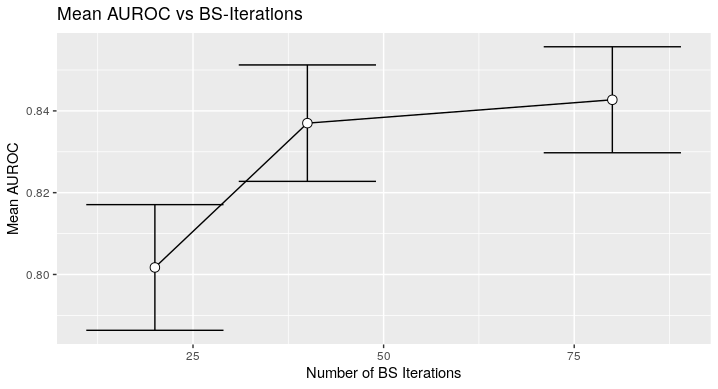
\includegraphics[width=8cm]{meanAUROCvsBSIterations}
		\centering
		\caption{Mean AUROC vs Bootstrap Iterations on M=50 datapoints}
		\label{fig:aurocBsIterations}
	\end{figure}

	\subsection{AUROC Score vs Number of Data Points}
	Figure \ref{fig:auroc_sample_size} shows that the Bagged GS algorithm is also sensible to the number of
	samples that our data contains; the experiment was done with a fixed number
	of \textbf{40 BS iterations} and a variation in our sample size \textbf{from 20 to 100 in
	steps of 10}. The experiment was repeated 3 times for each value of the sample
	size to also get an estimate on the mean and standard deviation of our
	results.
	% figure of aucroc - sample size 
	\begin{figure}[ht]
		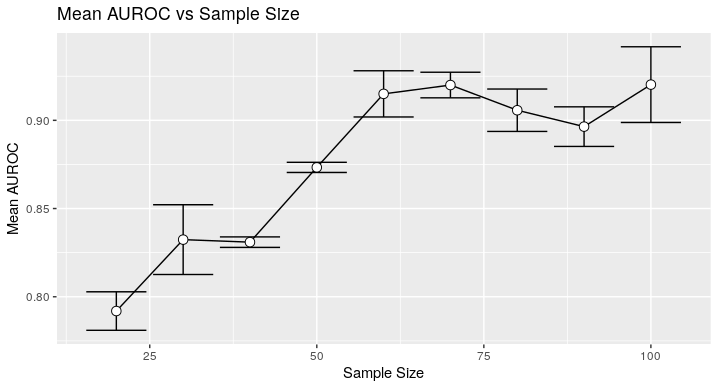
\includegraphics[width=8cm]{auroc_sample_size}
		\centering
		\caption{Mean AUROC vs Sample Size from M=20 to M=100}
		\label{fig:auroc_sample_size}
	\end{figure}
	We can observe that once our data goes beyond 60 data points, then an
	increase in sample size does not lead to a significant increase in AUROC
	metrics. All of our results after M=60 are within the estimated error. \\
	The experiment was run with a fixed number of 40 BS iterations because of our
	observed results on the first experiment. But it is also theoretically
	possible to further increase the AUROC of our models by increasing the number
	of BS iterations, due to lack of computing power we could not further explore
	this possibilities, our experiment took more
	than 3 hours to run on an 8 core i7-3.8 GHz modern CPU.

	\subsection{Bagged GS vs MCMC vs GS AUROC}
	In this experimental setting we did 3 experiments on data sets of varying
	size: \{20, 50, 100\} and subsequently compared the AUROC score obtained with
	Bagged GS with 40 iterations, MCMC with 20,000 iterations and vanilla GS. The
	experiment was repeated 5 times to get mean and standard deviation
	statistics. Afterwards we did a \textbf{t-test} on the obtained means resulting in
	table X.

	\section*{Appendix}

	\bibliographystyle{unsrt}
	\bibliography{biblio}

\end{document}

